%SourceDoc ../YourName-Dissertation.tex
%\vspace*{-80mm}
\chapter{Introduction} \label{chapter1:introduction}

\section{Motivation}
With an estimated total market of 2.8 million tons per year, specialty aluminas for non-metallurgical applications are arguably the most extensively used material in the field of ceramics. They are used in large volume applications such as high temperature refractories, technical ceramics, high voltage insulators, and functional fillers. The majority of Al$_{2}$O$_{3}$ applications use synthetic or specialty aluminas derived from Bayer feedstocks (Bayer aluminas), such as aluminum trihydrate (Al(OH)$_{3}$), smelter grade Al$_{2}$O$_{3}$ and others. Bayer aluminas are typically 99.0 - 99.9\% pure and contain Na$_{2}$O, CaO, Fe$_{2}$O$_{3}$, and SiO$_{2}$ impurities that originate from the bauxite ore and/or Bayer process reagents (e.g., NaOH). The vast majority of research on the sintering of Al$_{2}$O$_{3}$, however, focuses on ultrahigh purity ($\geq$ 99.99\%) aluminas derived from specialty feedstocks, such as ammonium alum (NH$_{4}$Al(SO$_{4}$)$_{2}$$\cdot$12H$_{2}$O), boehmite ($\gamma$-AlOOH) and aluminum chloride (AlCl$_{3}$). Due to the higher cost involved in producing the high purity chemicals and to maintain the purity during subsequent processes to obtain ultrahigh-purity aluminas, these powders are typically one to two orders of magnitude more expensive than Bayer aluminas. Therefore, for many industrial applications aluminas derived from the Bayer process constitute an overwhelming majority of the global market share of over 90\%.

While ultrahigh purity aluminas provide the purest platform from which to conduct fundamental sintering research, that research does not usually explore the types and amounts of impurities typical of Bayer aluminas. Commercial Bayer Al$_{2}$O$_{3}$ powders exist in a range of reactive grades that differ in the amount and types of these impurities, and additionally to impurities the manufacturer commonly adds MgO to commercial alumina powders since it is known for its beneficial effect during sintering. A fundamental understanding of the mechanisms of densification, grain growth and second phase formation is key for predicting and tailoring the sintering behavior and microstructure evolution of Bayer alumina powders based on their chemistry, and will provide valuable information to industrial users.

The purpose of this dissertation is to develop a fundamental, in-depth understanding about how the chemistry of commercial Bayer alumina powder affects sintering mechanisms, densification, grain growth, and the formation of second phases. Specifically, this dissertation will focus on investigating the effects and cross effects of MgO, Na$_{2}$O and SiO$_{2}$ on densification and microstructure evolution of Bayer aluminas, and provide insight into the fundamental mechanisms that are responsible for changes in sintering behavior. Furthermore, a model is developed to describe the dynamic development of grain boundaries during densification as a function of powder chemistry. It is crucial to understand the structure and chemistry of grain boundaries during sintering, as grain boundary diffusion is the dominant mechanism for mass transport. The methodology developed to analyze densification, microstructure evolution, sintering mechanisms, and grain boundaries during densification will serve as an example for investigating and tailoring the mechanisms of sintering in ceramic powders as a function of powder chemistry. Finally, the Master Sintering Curve approach is evaluated as a tool to identify powder chemistry effects on the sintering of Bayer alumina in a fundamental, predictive way.

\section{Sintering of Ceramics}
Sintering is the heat treatment of a particle mass, or high surface area powder, that results in a strength increase, reduction in surface area and, usually, densification. Sintering is used to fabricate bulk ceramic components and powder metallurgical parts \cite{Kang2004}, and can be divided into two main types; sold state sintering and liquid phase sintering. The difference between these two types of sintering is the absence or presence of a liquid phase, respectively, which results in fundamental differences in sintering mechanisms. 

The sintering process can be divided into three stages; initial, intermediate, and final stage sintering \cite{Kang2004}. Initial stage sintering accounts for the first few percent of densification, during which particles rearrange as a result of capillarity and contacts between particles form. The majority of densification occurs from $\sim$65 to $\sim$92\% relative density occurs and is termed intermediate stage sintering. During this stage the microstructure is characterized by pore channels along the grain edges. Little to no grain growth occurs during intermediate stage sintering since the presence of pore channels limits the mobility of grain boundaries. Intermediate stage solid state sintering is governed by densifying mechanisms, such as grain boundary and volume diffusion. In the presence of a liquid phase, grain boundary diffusion occurs by a solution-precipitation mechanism, where material from the particle - grain boundary interface dissolves into the liquid grain boundary phase, diffuses through the liquid grain boundary phase, and precipitates at sites of highest negative curvature, which is usually at the particle necks. In solid state sintering this diffusion process occurs by solid-state diffusion along the grain boundaries. At densities >92\% the pore channels that have formed during intermediate sintering close and form isolated pores on grain boundaries, which are eliminated during final stage sintering until full density is reached. Grain growth sets in after the closing of the pore channels at densities >92\% since grain boundaries with isolated pores are more mobile than grain boundaries with pore channels. As long as the mobility of the grain boundaries do not exceed the mobility of the pores, full density can be obtained. However, in many ceramic systems abnormal grain growth sets in at some point during sintering, and a limited number of grains grow abnormally fast, which results in a bimodal grain size distribution. Microstructures exhibit a few large grains, which are surrounded by a fine-grained matrix with grains that are orders of magnitude smaller than the large grains. The fast growth of these grains is due to a higher mobility of the grain boundaries of the large grains, which is much faster than the mobility of the pores. In this case pores cannot be removed fast enough from these grain boundaries, get trapped in the grains and remain in the final microstructure. Hence, the final density of a ceramic is often limited by the onset of abnormal grain growth. 

\section{Effects of Impurities and Dopants on the Sintering of Al$_{2}$O$_{3}$}

\subsection{MgO in Ultrahigh Purity Al$_{2}$O$_{3}$}

For a long time the performance and application of alumina as a technical ceramic was limited because it is known to exhibit abnormal grain growth. In 1961 Coble discovered that MgO-doping can suppress abnormal grain growth and high-density translucent alumina can be produced this way \cite{Coble1962a,Coble1962,Coble1961}. Since then numerous studies have attempted to understand the underlying mechanisms. Initially Coble proposed four possible mechanisms for the suppression of abnormal grain growth by MgO. As a first possible mechanism he proposed that spinel particles precipitate, pin the grain boundaries and prevent abnormal grain growth. The second mechanism he proposed was a solid-solution pinning mechanism, which assumed that MgO is preferentially adsorbed in the grain boundaries and inhibits abnormal grain growth by lowering the grain boundary mobility. The third proposed mechanism was that MgO could affect the pore shape and thereby increase the effect of pore pinning on grain boundary movement. The fourth proposed mechanism, which was the explanation Coble favored at that time, was that a minimum amount of time is required to nucleate abnormal grains after a critical density is reached, and that MgO increases the densification rate sufficiently to prevent the nucleation of abnormal grains. Since then multiple researchers have found arguments that support all of these mechanisms \cite{Bennison1990}. Jorgensen and Westbrook \cite{Jorgensen1964,Jorgensen1965} showed indirect evidence for MgO segregation to the grain boundaries and explained the effect of MgO on the sintering of Al$_{2}$O$_{3}$ by a solute pinning mechanism, where MgO influences the diffusion coefficient or surface energy through defect chemistry effects. Johnson and Coble \cite{Johnson1978} did not find evidence for MgO segregation in their experiments, and proposed that sintering kinetics change due to an increase in diffusion coefficient by the formation of a solid solution of MgO in Al$_{2}$O$_{3}$, which causes a change in grain growth and pore elimination rate. An alternative model was proposed by Heuer \cite{Heuer1979}, which assumed that MgO increases the pore mobility by increasing the surface diffusivity and, therefore, prevents pore-grain boundary breakaway and abnormal grain growth. 

A variety of the mechanisms described above were summarized in a segregation and precipitation map in unpublished work by Carry, Legros, Bowen, and Lartigue \cite{Zuo2013} as shown in Figure \ref{Ch1-figure:Figure1}. They proposed that when the MgO content in Al$_{2}$O$_{3}$ exceeds the maximum solubility of MgO in the Al$_{2}$O$_{3}$ lattice and a critical concentration of MgO in the grain boundaries, the excess MgO and Al$_{2}$O$_{3}$ form spinel precipitates. Schottky defects are formed below the solubility limit of MgO in the Al$_{2}$O$_{3}$ crystal, and the increased concentration of point defects facilitates diffusion and hence promotes the sintering by enhancing densification and grain growth. MgO concentrations that exceed the solubility of MgO in the Al$_{2}$O$_{3}$ lattice segregate to the grain boundaries, and when the solubility of MgO in the Al$_{2}$O$_{3}$ crystal and grain boundaries is exceeded, spinel precipitates form on the grain boundaries, which reduces the grain boundary mobility by a pinning mechanism, and thus inhibits grain growth. With increasing grain size the required MgO concentration for the formation of spinel decreases, as seen from the segregation and precipitation map in Figure \ref{Ch1-figure:Figure1}. The total area of the grain-boundary interface decreases with increasing grain size, and hence the critical concentration of MgO in the Al$_{2}$O$_{3}$ grain boundaries changes. While this proposed segregation precipitation map explains the observed segregation of MgO to grain boundaries and the precipitation of spinel, the key mechanism by which MgO improves the sintering of alumina cannot be identified. However, the segregation precipitation map implies that several of the described mechanisms may contribute to the effect of MgO on the sintering of alumina.

\subsection{Effects of Impurities during sintering of Al$_{2}$O$_{3}$}
After it was discovered that ppm levels of MgO are sufficient to drastically affect the sintering behavior of alumina \cite{Coble1961,Coble1962,Coble1962a}, there has been high academic and commercial interest in understanding how small concentrations of other dopants or impurities such as Na$_{2}$O, CaO, Fe$_{2}$O$_{3}$, and SiO$_{2}$ affect the sintering kinetics, density and microstructure evolution of alumina. An overwhelming amount of literature exists on how impurities, specifically SiO$_{2}$ and CaO, affect the sintering of ultrahigh purity aluminas, and the literature is in agreement that SiO$_{2}$ and CaO can form a liquid phase, which allows abnormal and anisotropic grain growth. Bae and Baik \cite{Bae1993a,Bae1997} showed that there is no abnormal grain growth in Al$_{2}$O$_{3}$, as long as the total impurity content is below 10 ppm, and it was realized that abnormal grain growth during sintering is not intrinsic to alumina, but depends on the presence of trace amounts of impurities on the ppm level, which form a liquid film on grain boundaries \cite{Bae1994,Handwerker1989,Gavrilov1999,Bennison1990}. By co-doping of Al$_{2}$O$_{3}$ with SiO$_{2}$ and CaO Bae and Baik \cite{Bae1993a} were able to show that a liquid forms during sintering as soon as the solubility of SiO$_{2}$ and CaO in Al$_{2}$O$_{3}$ is exceeded. They estimated the solubility of SiO$_{2}$ and CaO in Al$_{2}$O$_{3}$ to be 100 and 20 ppm, and that abnormal grain growth sets in after a critical thickness of the amorphous grain boundary has formed. This implies that impurity contents in commercial alumina powders with purity levels from 99.7 - 99.9\% are high enough to form a liquid phase during sintering, if glass-forming impurities are present, as demonstrated by Hansen and Philips \cite{Hansen1983}. Harmer \cite{Harmer1984} reported that even in 99.98\% pure alumina the impurity level is high enough for the formation of a liquid phase during sintering and it was concluded that abnormal grain growth could only be prevented by adding sintering additives such as MgO. 

\subsection{Effects of MgO on Liquid Phase Sintering of Al$_{2}$O$_{3}$}
Since it was established that abnormal grain growth is due to the presence of glass forming impurities in alumina, the role of MgO in alumina needed to be addressed in the context of these impurities, since MgO prohibits the deleterious effect of small amounts of liquid phase-forming impurities during sintering and facilitates the formation of a dense and homogeneous submicron microstructure. Several reasonable explanations can be found in the literature to explain this positive effect of MgO on the sintering behavior of Al$_{2}$O$_{3}$ containing small amounts of other impurities \cite{Bateman1989,Bennison1990}. Regardless of the presence of other impurities, the solute-pinning mechanism and the pinning-by-particle-precipitation mechanism are commonly accepted interpretations of the role of MgO on sintering of Al$_{2}$O$_{3}$ \cite{Soni1995,Bennison1983}. Bae and Baik \cite{Bae1994} suggested, that MgO acts as a glass modifier in glassy grain boundary films and changes the kinetics of dissolution precipitation mass transport by modifying the viscosity. Additionally, a reduction of the kinetics for dissolution into and precipitation from the liquid phase was considered as a key mechanism for sintering of MgO-doped alumina \cite{Bateman1989,Bennison1990}. 

Handwerker et al. \cite{Handwerker1989} proposed that MgO can increase the solubility of SiO$_{2}$ in Al$_{2}$O$_{3}$ by co-dissolving MgO, since the difference in size and charge of Mg$^{2+}$ and Si$^{4+}$ relative to Al$^{3+}$ in the alumina lattice can compensate each other. This co-dissolution mechanism is supported by the work by Gavrilov et al. \cite{Gavrilov1999}, who investigated the distribution of impurities in sintered Al$_{2}$O$_{3}$ by high-resolution scanning secondary mass spectrometry (SIMS). Figure \ref{Ch1-figure:Figure2} shows the SIMS maps of sintered Al$_{2}$O$_{3}$ singly doped with (a) 500 ppm MgO and (b) 1000 ppm SiO$_{2}$. Areas of high dopant concentrations appear bright, and in both cases it can be seen that the dopants segregate to the grain boundaries. Furthermore, they showed that if Al$_{2}$O$_{3}$ is co-doped with 500 ppm MgO and 1000 ppm SiO$_{2}$, both dopants segregate to the grain boundaries, but show a substantially higher MgO and SiO$_{2}$ concentration towards the grain center, as shown in the SIMS maps in Figure \ref{Ch1-figure:Figure3}. The authors concluded that the solubility of MgO and SiO$_{2}$ in Al$_{2}$O$_{3}$ is increased by co-doping via the following defect compensation mechanism:

%%
\begin{equation}
\label{Ch1-eq: eq1}
MgO + SiO_{2} \rightarrow Mg_{Al}^{'} + Si_{Al}^{\bullet} + 3O_{O}^{X}
\end{equation}
%%

%%
\begin{equation}
\label{Ch1-eq: eq2}
Mg_{Al}^{'} + Si_{Al}^{\bullet} + 3O_{O}^{X} \rightarrow \left[ Mg_{Al}^{'} - Si_{Al}^{\bullet} \right]^{X} + 3O_{O}^{X}
\end{equation}
%%

\noindent A similar reaction was proposed by Coble and Roy \cite{Roy1968} to explain a higher solubility of TiO$_{2}$ in Al$_{2}$O$_{3}$ when an equimolar amount of MgO is added. Gavrilov et al. \cite{Gavrilov1999} concluded that MgO increases the solubility of glass forming impurities in Al$_{2}$O$_{3}$ and therefore prevents the formation of a liquid phase during sintering. However, while they showed that there are higher Si and Mg concentrations in the alumina grains, they did not prove that no liquid phase exists in these samples. 

\subsection{Grain Boundaries During Sintering of Al$_{2}$O$_{3}$}
After the importance of grain boundaries for sintering of ceramics with ppm amounts of impurities and dopants was discovered, more recent literature has focused on developing general models based on grain boundary structures and chemistries to explain the sintering behavior and grain growth of ceramics. For example Harmer and his group \cite{Dillon2007a,Dillon2010,Dillon2007,Cantwell2014} proposed that impurities form thermodynamically stable grain boundary "phases", which they refer to as "complexions". Depending on the thickness of the adsorbed layer, i.e. the grain boundary thickness, they distinguish between six complexions: clean, monolayer, bilayer, multilayer, nanolayer and wetted, which can be either ordered or amorphous and show transitions from one to another during sintering. 

According to their model the mobility of the grain boundaries is determined by the type of complexion, which depends on impurity type and concentration, temperature and crystal orientation of adjacent crystals. During densification and grain growth impurities remain in the grain boundaries after the solubility in the crystal is exceeded. Grain boundaries can be sites for supersaturation during sintering because of the reduction of grain boundary area due to grain growth. The authors argue that there are only two possibilities for the excess impurities to reduce the free energy of the system; the formation of a new phase, or the transition to another complexion \cite{Dillon2010}. The predominance of either events depends on the relative activation energies. Since crystal planes of different orientation have different grain boundary or interface energies different complexions may co-exist in a microstructure. How many and what type of complexions coexist mainly depends on the temperature. Inhomogeneous impurity distribution may also be considered as a reason for the formation of different complexions. 

Using this concept the authors interpret the microstructure development of Al$_{2}$O$_{3}$ with different impurities. CaO impurities in Al$_{2}$O$_{3}$ can form calcium hexaluminate, which shows epitaxy on the basal planes of $\alpha$-Al$_{2}$O$_{3}$. The interface energy between the basal planes of $\alpha$-Al$_{2}$O$_{3}$ and calcium hexaluminate is low and therefore also the activation energy for formation. But for crystal planes with other orientations the activation energy for formation of calcium hexaluminate is high. Therefore, the theory suggests that complexion transitions are preferred on these planes and that the different grain boundary mobilities of the basal planes compared to all other planes lead to anisotropic abnormal grain growth, which is often observed in CaO containing alumina. 

SiO$_{2}$ in Al$_{2}$O$_{3}$ does not have a preferred crystal plane on which it can form precipitations with low interfacial energy. The activation energy for precipitation is high for all crystal orientations and, therefore, this system is interpreted to prefer complexion transitions rather than the formation of a new phase. It is stated that complexions with higher grain boundary mobilities form upon heating and that grain growth is enhanced. Dillon and Harmer's \cite{Dillon2007a,Dillon2008} interpretation for MgO in Al$_{2}$O$_{3}$ is that spinel precipitates are formed, and that this system behaves isotropically and exhibits low interface energies on several crystal planes. Therefore, it is stated that the activation energy for precipitation is low as well and that complexion transitions are prevented by the formation of spinel precipitates, or the precipitations occur uniformly throughout the microstructure. 

While this model can fundamentally explain the grain growth behavior in fully dense microstructures, it cannot explain observed differences in densification and how different chemistries, i.e. concentration and ratios of different impurities, and grain boundary structures affect the rate-limiting sintering mechanisms. 

A different model, based on the activation energy and the driving force for atoms to cross the grain boundary, was developed by Kang et al. \cite{Kang2004,Kang2009,Kang2016} to explain microstructure evolution in ceramics and metals. According to this model grains grow normal and an equiaxed microstructure develops if the critical driving force for grain boundary migration is zero and the grain interface is atomically rough. The critical driving force for grain boundary migration is determined by factors such as temperature, dopant concentration, and oxygen partial pressure, and if the critical driving force is zero then the step free energy, i.e. the additional surface energy created during nucleation and growth of grains (the ledges of the nucleus), has to be zero. If the critical driving force is not zero, then grains grow facetted, and if the maximum driving force, i.e. the driving force for the largest grains to grow, is larger than the critical driving force, then abnormal grain growth occurs. If the maximum driving force is much larger than the critical driving force, i.e. the driving force of many grains is larger than the critical driving force, many grains start growing fast ("abnormally") forming a microstructure that looks like a normally grown microstructure, and this is defined as pseudo-normal grain growth. If the maximum driving force is less than the critical driving force, then grain growth is stagnant, i.e. the microstructure does not change. 

Kang et al. \cite{Kang2016,Kang2009} investigated a variety of parameters such as partial pressure, temperature, dopants, and impurities for different material systems, but explained the microstructure evolution only qualitatively with the described model, and the majority of observations from experiments were fitted into the model rather than predicted by the model. For example, it is concluded that MgO lowers the step free energy of alumina since the addition of MgO to alumina results in a homogeneous and equiaxed microstructure \cite{Jo2006}. However, it is not explained why MgO lowers the step free energy, and why MgO is the only material that lowers the step free energy in that manner. Furthermore the model only takes into account the microstructural evolution in fully dense bodies and does not address densification.

\section{Sintering of Bayer Alumina}

\subsection{The Bayer Process}

The Bayer process is a hydrothermal precipitation process in which bauxite ore is digested in an aqueous solution of caustic soda (NaOH) at temperatures up to 230$^{\circ}$C and pressures up to 40 bar. Bauxite consists of a variety of minerals, including gibbsite (Al(OH)$_{3}$), boehmite ($\gamma$-AlO(OH)), diaspore ($\alpha$-AlO(OH)), goethite (FeO(OH)), haematite (Fe$_{2}$O$_{3}$), and kaolinite (Al$_{2}$Si$_{2}$O$_{5}$(OH)$_{4}$). During digestion in NaOH the Al-containing minerals form NaAl(OH)$_{4}$, which dissolves as a complex. Fe- and Si-containing minerals and other accessory minerals are insoluble under these conditions and can be separated as red mud. The temperature of the sodium aluminate solution is decreased to 50-70$^{\circ}$C and the addition of $\gamma$-Al(OH)$_{3}$ seed crystals results in the precipitation of $\gamma$-Al(OH)$_{3}$ from the solution. Heat treatment and calcination of the $\gamma$-Al(OH)$_{3}$ at 1100 - 1200$^{\circ}$C leads to the formation of $\alpha$-Al$_{2}$O$_{3}$.

SiO$_{2}$ and Fe$_{2}$O$_{3}$ are the main components of the Bauxite ore, additionally to Al$_{2}$O$_{3}$, and hence low concentrations of SiO$_{2}$ and Fe$_{2}$O$_{3}$ are present in the final powder. Additional SiO$_{2}$ impurities may originate from the milling media that is used by the manufacturer to grind the calcined powder to the desired particle size \cite{Compson2013,Bennison1990}. Na$_{2}$O impurities result from the digestion of the bauxite in NaOH and the consequent precipitation of Al(OH)$_{3}$ crystals from the NaAl(OH)$_{4}$ solution. Small amounts of Na$_{2}$O are precipitated within the Al(OH)$_{3}$ crystals \cite{Compson2013}. To remove NaOH from the powder surface, the Al(OH)$_{3}$ is washed after precipitation. However, small amounts of NaOH or rather Na$_{2}$O after calcination, remain on the powder surface. Hence, Na$_{2}$O impurities are either distributed on the surface, or entrapped in the alumina grains in Bayer process alumina powders. Other impurities such as gallium, calcium and magnesium originate from accessory minerals in the bauxite \cite{Bennison1990}.

\subsection{Influence of Na$_{2}$O and SiO$_{2}$ on the Sintering Behavior of Al$_{2}$O$_{3}$}
The Bayer process illustrates that alumina powders obtained by this process inevitably contain trace amounts of impurities, such as Na$_{2}$O and SiO$_{2}$. Despite the extensive use of Bayer alumina there are relatively few published studies on the effects of Na$_{2}$O on its sintering. Sumita and Bowen reported on the effect of adding 1 wt.\% Na$_{2}$O to a high purity alumina powder (Sumitomo, AKP-HP) \cite{Sumita1988}. However, they determined that only $\sim$8 ppm Na$_{2}$O was present in the alumina after sintering at 1400$^{\circ}$C for 2 h, without additional details to explain the large discrepancy between the doping concentration and the amount determined by inductively coupled plasma (ICP) spectrometry after sintering. Smothers and Reynolds \cite{Smothers1954} investigated the influence of 1 wt.\% of different additives on the sintering of 99.3\% pure alumina (Alcoa A-11) and showed that Na$_{2}$CO$_{3}$ or NaF retard sintering and inhibit grain growth. 

Cahoon and Christensen \cite{Cahoon1956} reported a deleterious effect of Na$_{2}$O on the sintering of alumina as well. They added between 0.03 and 5.9 wt.\% Na$_{2}$O to their alumina powder (Alcoa A-14, no purity specifications given) and heated the samples in a 5 days cycle (2 days heating, 3 days cooling) to temperatures between 1600$^{\circ}$C and 1835$^{\circ}$C for 1 h. A very strong retardation of sintering and inhibition of abnormal grain growth was reported for increasing Na$_{2}$O concentration. They observed cracking of their samples and inferior compressive strengths and suggested that this deleterious effect might be due to the formation of $\beta$- or $\xi$-Al$_{2}$O$_{3}$. They also studied the effect of SiO$_{2}$ on the sintering of Al$_{2}$O$_{3}$ and reported a "moderately deleterious effect" of SiO$_{2}$. They claim that it strongly inhibits abnormal grain growth at concentrations as low as 0.1\% and that this effect is enhanced with increasing SiO$_{2}$ content. They reported that the deleterious effect of Na$_{2}$O was moderated in Na$_{2}$O/SiO$_{2}$ co-doped Al$_{2}$O$_{3}$.

Louet et al. \cite{Louet2005a} studied the effect of Na$_{2}$O and SiO$_{2}$ doping on densification and microstructure evolution of a Bayer process alumina (Rhone-Poulenc, P172SB), containing 550 ppm Na$_{2}$O, 770 ppm SiO$_{2}$, 1010 ppm MgO, 600 ppm CaO and 115 ppm Fe$_{2}$O$_{3}$. Na$_{2}$O and SiO$_{2}$ levels were adjusted by adding CH$_{3}$COOH-Na and silica gel. When they added Na$_{2}$O, the concentrations in the samples after sintering for 2 h at 1540$^{\circ}$C, as measured by ICP spectrometry, were less than 50\% of the targeted amount, and they explained this difference by the low vaporization temperature of Na$_{2}$O \cite{Louet2005a}. Louet et al. concluded that Na$_{2}$O slows the sintering process and decreases the sintered density from 98 to 97\% for Na$_{2}$O concentrations of 550 ppm and 1150 ppm, respectively, when sintered at 1540$^{\circ}$C for 2h. The authors reported that a high level of Na$_{2}$O results in a fine, homogeneous microstructure. They observed a drop in grain size from 4 - 5 $\mu$m to 3 $\mu$m when exceeding 1000 ppm Na$_{2}$O. This work also showed that increasing SiO$_{2}$ concentration from 770 ppm to as high as 1500 ppm in the presence of Na$_{2}$O does not affect the final density but does cause anisotropic grain growth. Even though one can see an increase in grain size but no abnormal grain growth as the SiO$_{2}$ concentration increases in the presented micrographs, the authors state that increasing the SiO$_{2}$ concentration has no effect on the average grain size but leads to abnormal grain growth. As noted by the authors, these results are difficult to interpret in terms of Na$_{2}$O and SiO$_{2}$ effects due to the large number and high concentrations of impurities in the as-received powder. 

Compson et al. \cite{Compson2013} investigated the effect of SiO$_{2}$ and Na$_{2}$O concentration on the sintering behavior of alumina. They chose four commercial alumina powders with similar specific surface areas, particle diameter and particle distributions. All powders were 99.8\% pure, but showed different concentrations for the single impurities. Particularly, the Na$_{2}$O and SiO$_{2}$ concentrations varied from 0.02 to 0.1\% and 0.01 to 0.04\%, respectively. Using dilatometry they showed that the four powders exhibit different shrinkage, sintering and densification behavior in the temperature range from 1150$^{\circ}$C to 1500$^{\circ}$C. They concluded that SiO$_{2}$ has a deleterious effect on the sintering of Al$_{2}$O$_{3}$, but they could not detect an influence of Na$_{2}$O.

This literature survey shows that there is some disagreement about whether ppm levels of Na$_{2}$O and SiO$_{2}$ have a positive, negative, or no effect on sintering of alumina, and unfortunately none of the literature reports investigated fundamental mechanisms that would explain their observations. While most authors acknowledged the presence of other impurities and dopants, such as MgO, their effect and possible cross effects with other impurities or dopants were not considered. The lack of understanding of this system was the motivation to investigate the fundamental mechanisms that are responsible for changes in sintering behavior as a function of powder chemistry in Bayer process-derived Al$_{2}$O$_{3}$.

The chapters of this dissertation have either been published, submitted for publication, or will be submitted for publication in peer-reviewed scientific journals. As a result some degree of self-plagiarism was necessary to construct this dissertation.

\newpage
%%%
\begin{figure}[H]
	\centering
	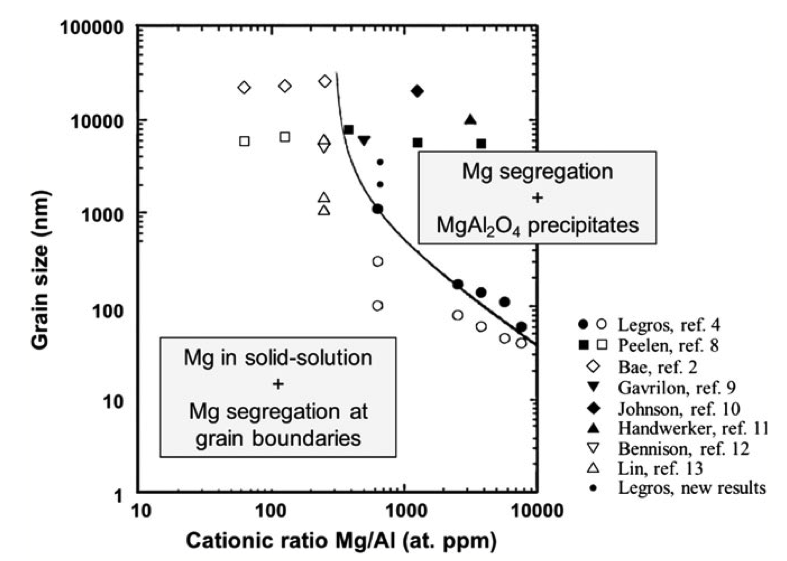
\includegraphics{Chapter-1/Figures/Figure1.png}
	\caption{Segregation and precipitation map of MgO-doped alumina based on the results in the literature \cite{Zuo2013}.}
	\label{Ch1-figure:Figure1}
\end{figure}
%%%

\newpage
%%%
\begin{figure}[H]
	\centering
	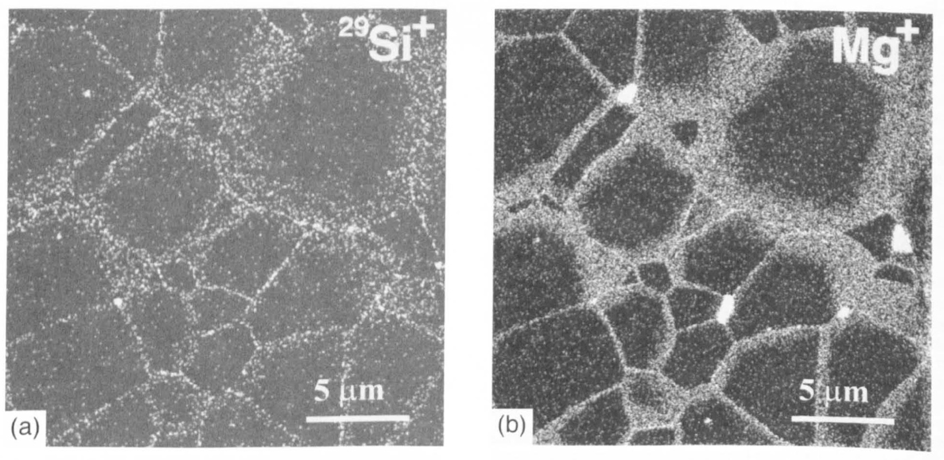
\includegraphics{Chapter-1/Figures/Figure2.png}
	\caption{SIMS maps of Al$_{2}$O$_{3}$ doped with 500 ppm MgO (a) and 1000 ppm SiO$_{2}$ (b). Samples were sintered for 8 h at 1650$^{\circ}$C \cite{Gavrilov1999}.}
	\label{Ch1-figure:Figure2}
\end{figure}
%%%

\newpage
%%%
\begin{figure}[H]
	\centering
	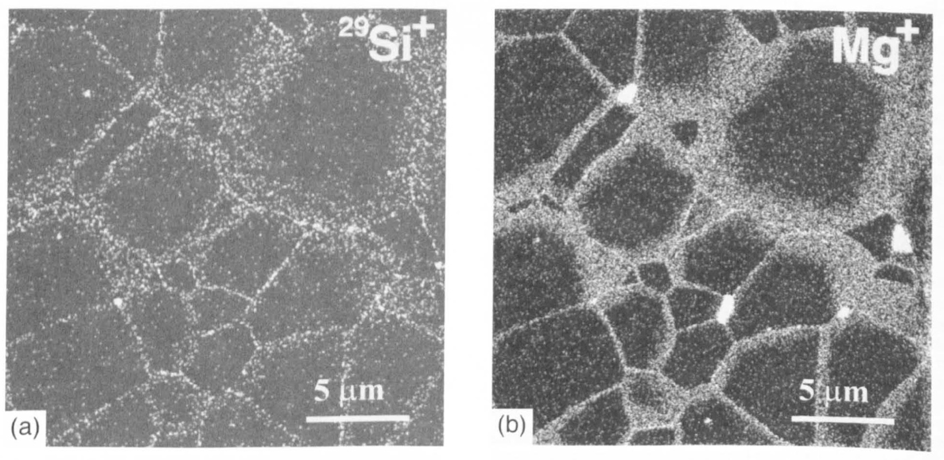
\includegraphics{Chapter-1/Figures/Figure3.png}
	\caption{SIMS maps of Al$_{2}$O$_{3}$ co-doped with 500 ppm MgO and 1000 ppm SiO$_{2}$ and sintered at 1650$^{\circ}$C for 8h. (a) shows the distribution of SiO$_{2}$, (b) the distribution of MgO in the same samples \cite{Gavrilov1999}.}
	\label{Ch1-figure:Figure3}
\end{figure}
%%%
